\documentclass[class=article, crop=false]{standalone}
\usepackage[subpreambles=true]{standalone}
\usepackage{import}
\usepackage[T1]{fontenc}
\usepackage[utf8]{inputenc}
\usepackage[english, danish]{babel}
\usepackage{graphicx,wrapfig,lipsum}

\begin{document}
    På Pakkediagrammet, Figur~\ref{fig:pakkediagram}, kan det tydeligt ses at vores overordnede opdeling i projektstrukturen er lavet ud fra Model-View-Controller design mønstret. Dette har vi valgt at gøre for nemmere at kunne adskille data (model-laget), logikken (controller-laget) og spillebrættet (View-laget). Denne opdeling er almindeligt anerkendt og findes overskuelig, så det egner sig til vedligeholdelse og videreudvikling af programmet.

    \begin{figure}[H]

         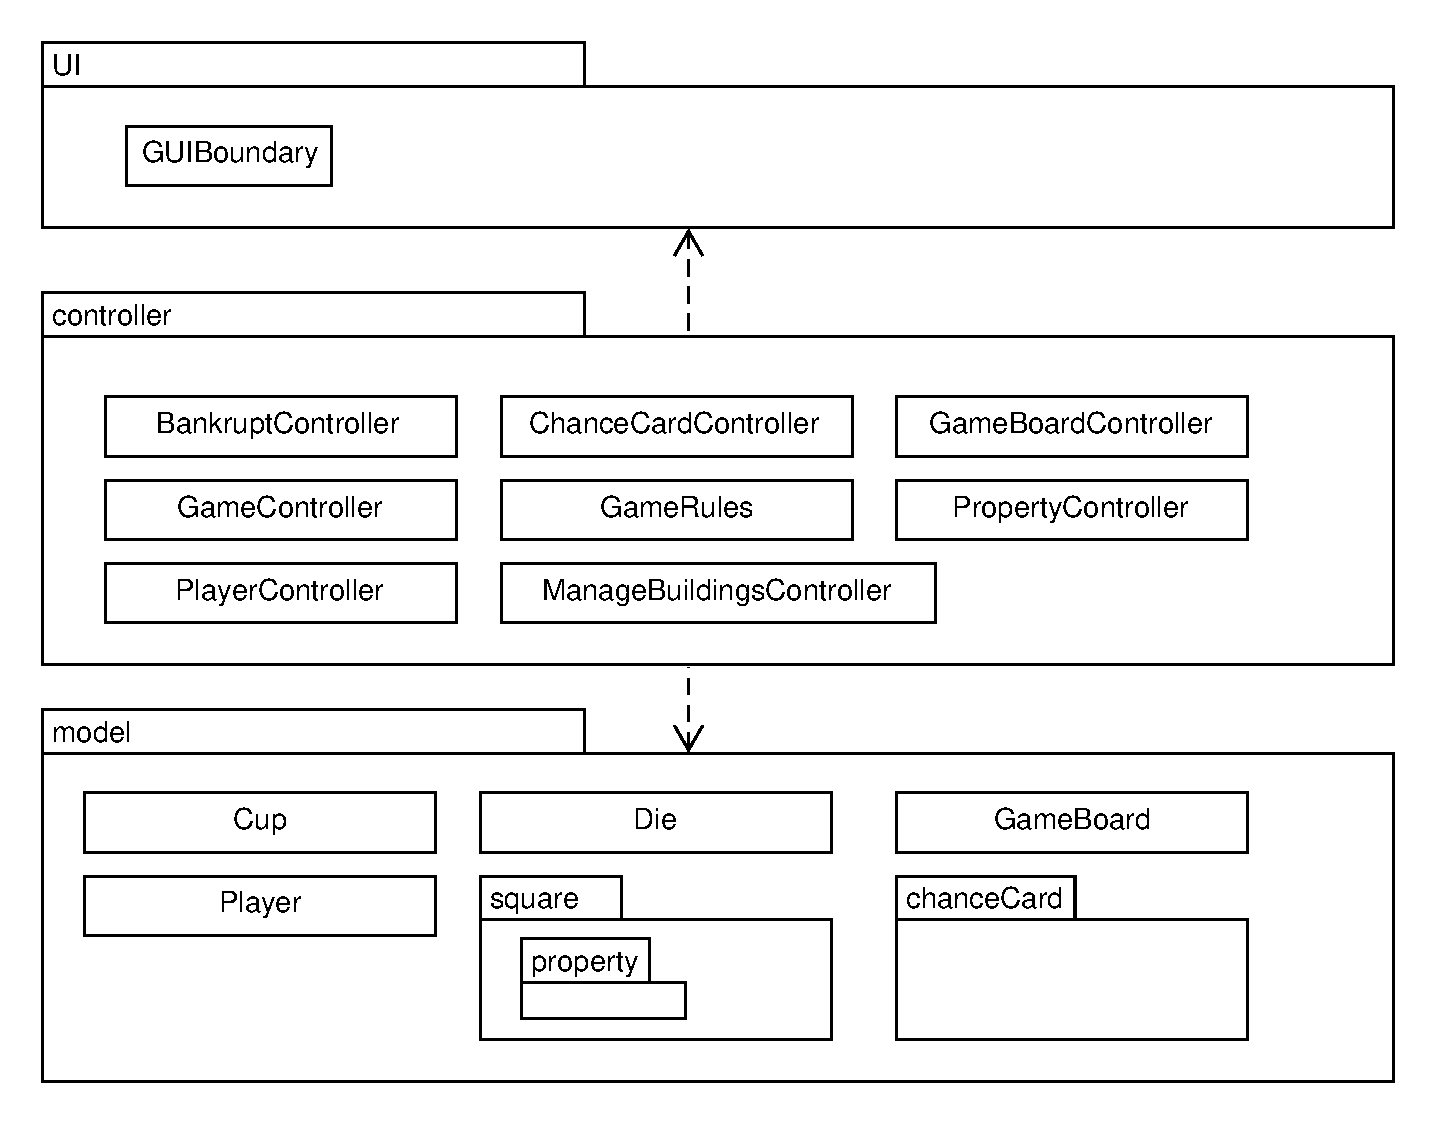
\includegraphics[scale=0.7]{diagrams/pakke_diagram.pdf}

        \caption{Pakkediagrammet over systemet}\label{fig:pakkediagram}
    \end{figure}

\end{document}